\documentclass[a4paper,norsk]{article}
\usepackage{preamble}
\usepackage{amsmath}
\begin{document}
\maketitle


As a strategy to approximate a function f with a function g, one can use the well least squares method to make the quation
\begin{align*}
||f - g|| = \sqrt{\int_0^1 (f(t) - g(t) )^2 dt }	
\end{align*} 
be as small as possible.
We define ${N_1(x), N_2(x), ..., N_n(x)}$ to be a basis for the set of polynomials of degree at most n-1. For a chosen set of basis, we want to 
find a "best fit" polynomial to f, such that $||\sum_{j=1}^n c_j N_j - f ||$ is minimized with respect to the coefficients $c_j$
From the least squares approximation, we end up with the system
\begin{align*}
\mathbf{c^T N c} -2\mathbf{b^T c} + ||f||^2
\end{align*}
Where \textbf{N} is the matrix with entries $\langle N_i, N_j \rangle$ and \textbf{b} is the vector with entries $\langle N_j, f \rangle$ 

\section*{Problem 1}
First we want to show that matrix \textbf{N} is positive definite.  A n × n real matrix M defined as positive definite if the scalar $ x^{T}M x$ is positive for every choice of a non-zero column vector x of dimention n. A natural extention of the definition would be to consider the system $\mathbf{c^TNc}$.
\begin{align*}
c^TNc = c_i \langle N_i, N_j \rangle c_j = \int_0^1 \sum_{i=1}^n c_i N_i \sum_{j=1}^n c_j N_j dx = \int_0^1 p(x)^2 dx  \geq 0
\end{align*}

\section*{Problem 2}
Computing the gradient of the expression $\mathbf{c^T N c} -2 \mathbf{b^t c} + ||f||^2 $ with respect to $c_i$ we get

\begin{align*}
\frac{\partial}{\partial c_i} \Big[ \mathbf{c^T N c} -2 \mathbf{b^t c} + ||f||^2\Big] = 2\mathbf{Nc} - 2\mathbf{b^t} \\
\end{align*}
From simple observations of the least squares method, one can see that the trend of $||f - g|| = \sqrt{\int_0^1 (f(t) - g(t) )^2 dt }$ will follow some sort of second order polynomial. Hence the minimal
extreme point for the smallest error will be found for 
$\frac{\partial}{\partial c_i} \Big[ \mathbf{c^T N c} -2 \mathbf{b^t c} + ||f||^2\Big] = 0 $ hence $\mathbf{Nc} = \mathbf{b}$ 

\section*{Problem 3}
Defining $N_j(x) = x^{j-1} \hspace{2mm} 1 \leq j \leq n$, we are ought to show that the matrix \textbf{N} really is the Hilbert matrix with entries $\frac{1}{i + j - 1}$
\begin{align*}
\mathbf{N} = \langle N_i, N_j \rangle = \int_0^1 x^{i - 1} x^{j - 1} dx = \int_0^1 x^{i + j- 2} dx = \Big[\frac{1}{i+j+1} x^{i+j+1} \Big]_0^1 = \frac{1}{i+j+1} 
\end{align*}

\section*{Problem 4}
Showing that $P_n(x) = x^n + \sum_{k=0}^{n-1} c_k x^k$ is orthogonal to $1, x, ...., x^{n-1}$ on [-1, 1], we require that $\langle P_n,  N_j\rangle = 0$. I tried to do this integration but was unable to show this, so I assume I have something wrong in my calculations\\
But let us assume that $\langle P_n,  N_j\rangle = 0$, then using the same arguments as in problem 3, we have to solve the linear system $\mathbf{Nc = b}$, where b in this case will be a contribution from the $x^n$ term.
\begin{align*}
&\langle P_n,  N_j\rangle = \int_{-1}^1  \Big[x^n + \sum_{k=0}^{n-1} c_k x^k\Big]x^{j-1} dx = 0 \\
 &\int_{-1}^1 \sum_{k=0}^{n-1} c_k x^k x^{j-1} dx = -\int_{-1}^1  x^n x^{-j} dx = -\langle x^n, x^{j-1}\rangle = \mathbf{Nc} = \mathbf{b}  \\
 &\mathbf{b} = -\langle x^n, x^{j-1}\rangle = -\Big[\frac{x^{n+j} }{n+j} \Big]_{-1}^1  = 
 \begin{cases} 
      0 \hspace{2mm} \text{if n + j is even } \\
      -\frac{2}{n+j} \hspace{2mm} \text{if n + j is odd}
   \end{cases}
\end{align*}

\section*{Problem 6}
\begin{figure}[h!]
	\centering
	\caption*{\textbf{First 10 Legendre polynomials}}
	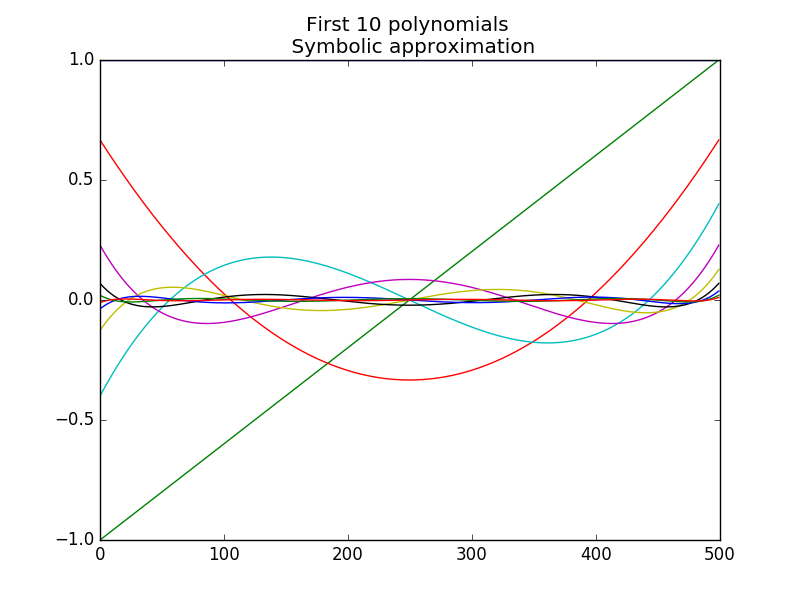
\includegraphics[scale=0.36]{sym10.png}
	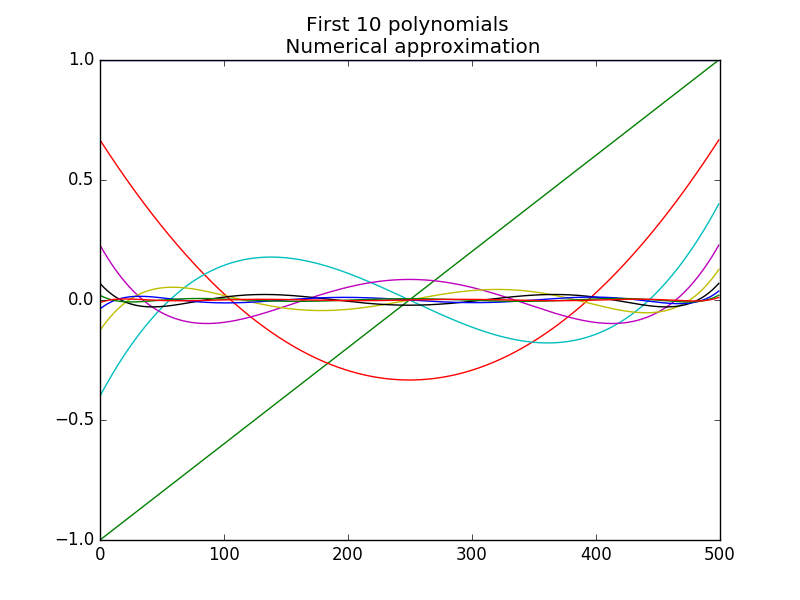
\includegraphics[scale=0.36]{num10.png}
\end{figure}

\newpage
\section*{Problem 7}
Examening the calculations for different n, the first problem I run into is the computation of the condition number for the symbolic expression. Allerady for the Legendre polynomial n = 9, python is unable to represent it.

For the numerical condition number we see a cleary increasing trend as we approach $n > 15$
\begin{lstlisting}[style=terminal]
FOR N = 0.000000 CONDITION NUMBER NUMERIC  1.0000
FOR N = 1.000000 CONDITION NUMBER NUMERIC  1.0000
FOR N = 10.000000 CONDITION NUMBER NUMERIC  20.2153
FOR N = 14.000000 CONDITION NUMBER NUMERIC  90.7308
FOR N = 15.000000 CONDITION NUMBER NUMERIC  132.8401
FOR N = 18.000000 CONDITION NUMBER NUMERIC  421.0646
FOR N = 21.000000 CONDITION NUMBER NUMERIC  1350.1202
FOR N = 23.000000 CONDITION NUMBER NUMERIC  2954.0884
FOR N = 24.000000 CONDITION NUMBER NUMERIC  4264.7171
\end{lstlisting}

Visually our computations seems reasonable until we reach the 24 Legendre polynomial. The dataplots clearly shows that we are starting to get in throuble representing the polynomials numerically. This combined with the increasing condition number for the matrix \textbf{P}, this will not yield accurate results for increasing n. One of the main reasons for this is the fact that for higher n, the indices of the matrix \textbf{N} will tend to go to zero as per definition of the inner product from 
$\mathbf{exercise}$ 4. Hence our system will tend to a singular system, which will effect our system in our numerical linear solvers.
\begin{figure}[!ht]
	\centering
	\caption*{\textbf{First indication of trouble}}
	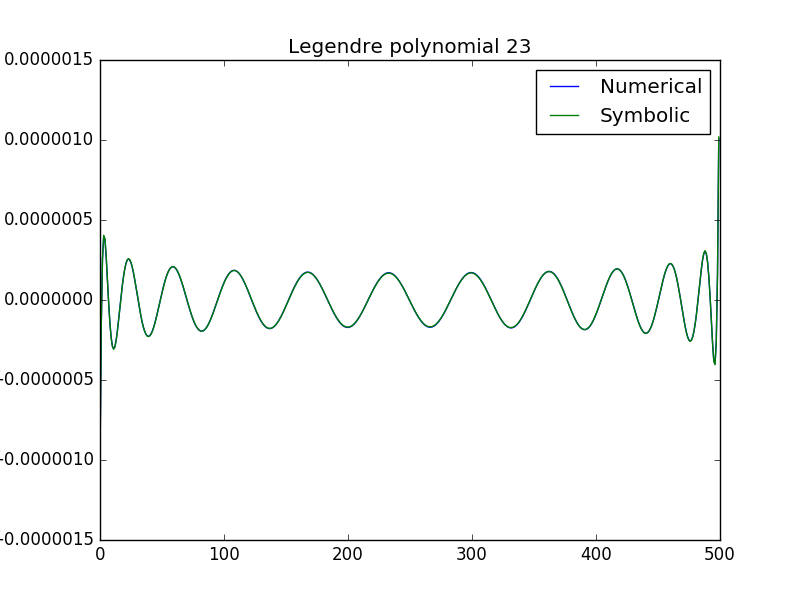
\includegraphics[scale=0.36]{n23.png}
	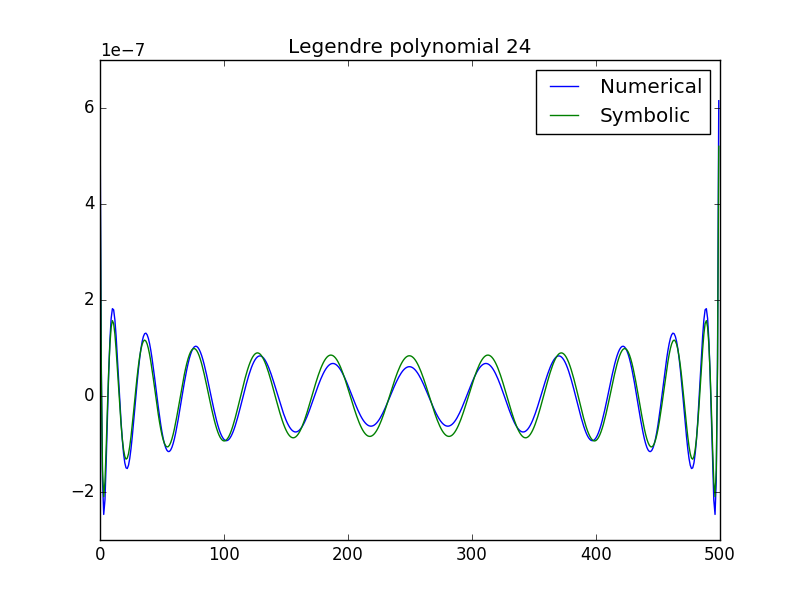
\includegraphics[scale=0.36]{n24.png}
\end{figure}

\newpage
\section*{Problem 8}
In this exercise we are supposed to show that $\frac{d^n(x^2 -1 )^n}{dx^n}$ is orthogonal to all functions$1, x, ...,x^{j}$ $1 \leq j < n$
on $[-1, 1]$. By inner product and integration by parts we get the following relation
\begin{align*}
\langle \frac{d^n(x^2 -1 )^n}{dx^n}, x^{j}\rangle &= \int_{-1}^{1} \frac{d^n(x^2 -1 )^n}{dx^n} x^{j} dx = 
\Big[\frac{d^{n-1}(x^2 -1 )^n}{dx^{n-1}}, x^{j} \Big]_{-1}^{1} - \int_{-1}^{1} \frac{d^{n-1}(x^2 -1 )^n}{dx^{n-1}}, jx^{j-1} dx \\
&= - \Big[\frac{d^{n-2}(x^2 -1 )^n}{dx^{n-2}}, jx^{j} \Big]_{-1}^{1} + \frac{d^{n-2}(x^2 -1 )^n}{dx^{n-2}}, j(j-1)x^{j-2} dx
\end{align*}
Observing that our boundary integrations equals zero, we get the following relation after the i´th step of integration by parts
\begin{align*}
\langle \frac{d^n(x^2 -1 )^n}{dx^n}, x^{j}\rangle = \int_{-1}^1(-1)^i\frac{d^{n-i}(x^2 -1 )^n}{dx^{n-i}} \frac{j!}{(j-i)!} x^{j-i} dx
\end{align*}
As a result we observe that from the n`th integration by parts, our polynomial $x^{j} \hspace{2mm} 1 \leq j < n$ turns zero, hence the orthogonality is shown \\
Further why must we have  $Pn(x) = \frac{n!}{2n!} \frac{d^n(x^2-1)^n}{dx^n}$ \\

If we rewind ourselfs to \textbf{exercise 4} we proved that a polynomial on the form $Pn(x) = x^n + \sum_{k=0}^{n-1}c_k x^k$ is orthogonal to 
$x^j \hspace{2mm} 0 \leq j < n$. Expanding our polynomial $Pn(x)$ in this exercise (leaving the fractorial for now) one could say we have apolynomial on the form
\begin{align*}
\frac{d^n(x^2-1)^n}{dx^n} = \frac{d^n}{dx^n} \Big(x^{2n} + c_{2n-1}x^{2n-1} + .. + c_{n}x^{n} + ... + c_{1}x + c_{0} \Big)	
\end{align*} 
We strictly don`t know the constants due to the general n, but we know they are based on the choice of some n.
Firstly one observes that for every polynomial $x^j \hspace{2mm} j < n$ will equal zero due to the degree of the derivate. Further we can show in general 
that the derivation of a polynomial $x^{2n}$ can be generalized as 
\begin{align*}
\frac{d^n}{dx^n}x^2n \hspace{2mm} \rightarrow 2nx^{2n-1} \hspace{2mm} \rightarrow 2n(2n-1)x^{2n-2}\hspace{2mm} \rightarrow \frac{2n!}{n!}x^n
\frac{d^n}{dx^n}x^{2n-1} \hspace{2mm} \rightarrow (2n-1)x^{2n-2}\hspace{2mm} \rightarrow \frac{(2n-1)!}{(n-1)!}x^n
\end{align*}
Hence from our argumentation we are left with a polynomial on the same form as in $Exercise 4$ but with the term factorial term. Now by using the left out factorial
$\frac{n!}{2n!}$, we eliminate the $\frac{n!}{2n!}$ for $x^{2n}$ and we have reduced the polynomial to one of the form from \textbf{Exercise} 4. By this we know that we
can define $\mathbf{Nc=b} $ to solve our least squares problem, but now
\textbf{N} is the matrix with entries $\langle P_i, P_j \rangle$ and \textbf{b} is the vector with entries $\langle P_j, f \rangle$ 

\newpage
\section*{Problem 9}
So we have the initial expression $\langle \frac{d^n(x^2 -1 )^n}{dx^n}, \frac{d^n(x^2 -1 )^n}{dx^n} \rangle $. Integration by parts yields

\begin{align*}
\langle \frac{d^n(x^2 -1 )^n}{dx^n}, \frac{d^n(x^2 -1 )^n}{dx^n} \rangle  = 
\Big[ \frac{d^{n-1}(x^2 -1 )^n}{dx^{n-1}} \frac{d^n(x^2 -1 )^n}{dx^n} \Big]_{-1}^1 
- \int_{-1}^1 \frac{d^{n-1}(x^2 -1 )^n}{dx^{n-1}} \frac{d^{n+1}(x^2 -1 )^n}{dx^{n+1}} dx \\
\end{align*}
In General we have the relation for the i´th integration by parts
\begin{align*}
\langle \frac{d^n(x^2 -1 )^n}{dx^n}, \frac{d^n(x^2 -1 )^n}{dx^n} \rangle  = 
(-1)^i \int_{-1}^1 \frac{d^{n-i}(x^2 -1 )^n}{dx^{n-i}} \frac{d^{n+i}(x^2 -1 )^n}{dx^{n+i}} dx
\end{align*}

Now choosing $i = n$ we get 
\begin{align*}
\langle \frac{d^n(x^2 -1 )^n}{dx^n}, \frac{d^n(x^2 -1 )^n}{dx^n} \rangle  = 
(-1)^n \int_{-1}^1 (x^2 -1 )^n \frac{d^{2n}(x^2 -1 )^n}{dx^{2n}} dx \\
 = (-1)^n (2n!) \int_{-1}^1 (x^2 -1 )^ndx
\end{align*}




\end{document}

